\subsection{30. Замкнутость конечных преобразований относительно композиции.}

\Th Если $\psi_1:\Sigma^* \rightarrow \Gamma^*$ и $\psi_2:\Gamma^* \rightarrow \Pi^*$ -- КП, то $\psi = \psi_2 \circ \psi_1$ -- КП

\Proof
$\psi_1=L(M_1)$, $M_1$ -- КПтель : $\angles{Q, \Sigma, \Gamma, \Delta_Q, q_0, F_Q}$

 $\psi_1=L(M_1)$, $M_1$ -- КПтель : $\angles{P, \Gamma, \Pi, \Delta_P, p_0, F_P}$

Тогда $M_{comp} = \angles{Q \times P, \Sigma, \Pi, \Delta', (q_0,p_0), (F_Q\times F_P)}$

Сразу отметим, что все переходы в $\psi_1, \psi_2 \; : \; |u| + |v| = 1$. Тогда положим:
\begin{figure}[h!]
    \centering
    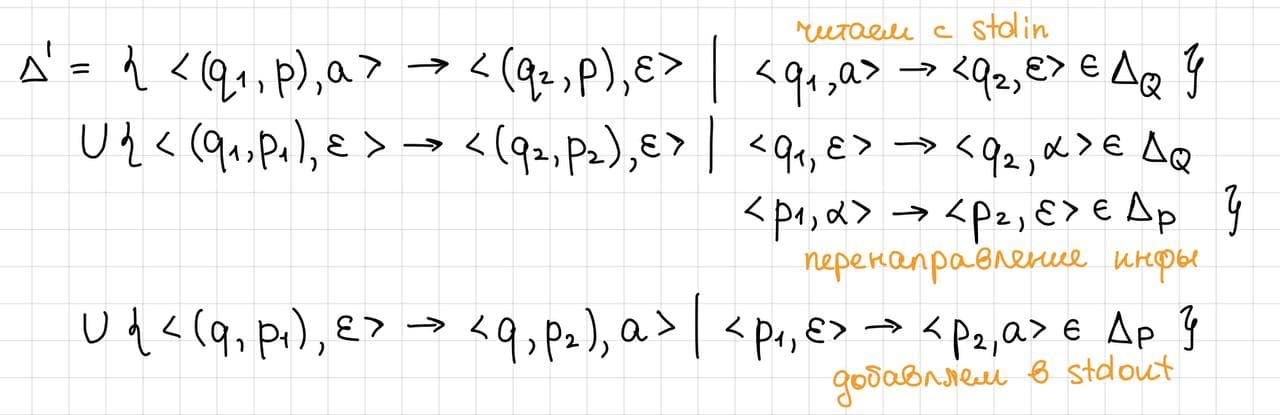
\includegraphics[scale=0.6]{images/delta.jpg}
\end{figure}

\Lemma $\angles{(q_1,p_1), u, \varepsilon} \vdash_{M_{comp}} \angles{(q_2,p_2), \varepsilon, v} \Longleftrightarrow \exists w\in \Gamma^* : \angles{q_1, u, \varepsilon} \vdash_{M_Q} \angles{q_2,\varepsilon, w}$ и $\angles{p_1, w, \varepsilon} \vdash_{M_P} \angles{p_2,\varepsilon, v}$

$\Longrightarrow$: индукция по длине вывода в $M_{comp}$. В переходе делаем разбор случаев: $(a, \varepsilon), \ (\varepsilon, \varepsilon), \ (\varepsilon, a)$

\Proof
\textit{База:} 0 шагов

$\angles{(q_1,p_1), u, \varepsilon} \vdash_0 \angles{(q_2,p_2), \varepsilon, v}$. 

Значит, $q_1 = q_2, p_1 = p_2, u = \varepsilon, v = \varepsilon$\\

\textit{Переход:}

Мы имеем следующее: $\angles{(q_1,p_1), u, \varepsilon} \vdash \angles{(q_3,p_3), u', v'} \vdash_1 \angles{(q_2,p_2), \varepsilon, v}$

Далее у нас есть 3 случая в зависимости от того, какой был последний переход (они соответствуют трем множествам из объединения для $\Delta$):

\begin{enumerate}
    \item Можем сделать несколько выводов:
    \begin{enumerate}
        \item $u' = a$
        \item $v' = v$
        \item $p_3 = p_2$
        \item $\angles{q_3, a} \rightarrow \angles{q_2, \varepsilon} \in \Delta_p$ (исходное $\Delta$)
    \end{enumerate}
    
    Поэтому $\angles{(q_1, p_1), u''a, \varepsilon} \vdash \angles{(q_3, p_2), a, v} \Rightarrow \angles{(q_1, p_1), u'', \varepsilon} \vdash \angles{(q_3, p_2), \varepsilon, v} $. 
    
    Значит, по предположению индукции, $\exists w: \angles{q_1, u'', \varepsilon} \vdash \angles{q_3, \varepsilon, w}$ и $\angles{p_1, w, \varepsilon} \vdash \angles{p_2, \varepsilon, v}$. (Получили одну из нужных выводимостей).
    
    А еще $\angles{q_1, u''a, \varepsilon} \vdash \angles{q_3, a, w} \vdash \angles{q_2, \varepsilon, w}$.
    
    \item Можем сделать несколько выводов:
    \begin{enumerate}
        \item $u' = \varepsilon$
        \item $v' = v$
        \item $\exists \alpha \in \Gamma:$ 
        
        $\angles{q_3, \varepsilon} \rightarrow \angles{q_2, \alpha}$ и $\angles{p_3, \alpha} \rightarrow \angles{p_2, \varepsilon}$
    \end{enumerate}
    
    Из $\angles{(q_1, p_1), u, \varepsilon} \vdash \angles{(q_3, p_3), \varepsilon, v}$ по предположению индукции следует, что
    
    $\exists w \in \Gamma^*:$
    
    $\angles{q_1, u, \varepsilon} \vdash \angles{q_3, \varepsilon, w}$ -- (1)
    
    $\angles{p_1, w, \varepsilon} \vdash \angles{p_3, \varepsilon, v}$ -- (2)
    
    Применим к (1) результаты вывода номер 3 и получим:
    $\angles{q_3, \varepsilon, w} \vdash \angles{q_2, \varepsilon, w\alpha}$
    
    А, воспользовавшись уже второй выводимостью из вывода номер 3 получим:
    
    $\angles{p_1, w\alpha, \varepsilon} \vdash \angles{p_3, \alpha, v} \vdash \angles{p_2, \varepsilon, v}$
    
    Из существования $w\alpha$ -- переход выполнен.
    \item Можем сделать несколько выводов:
    \begin{enumerate}
        \item $q_3 = q_2$
        \item $v = v'a$
        \item $u' = \varepsilon$
        \item $\angles{p_3, \varepsilon} \rightarrow \angles{p_2, a} \in \Delta_p$
    \end{enumerate}
    
    Из $\angles{(q_1, p_1), u, \varepsilon} \vdash \angles{(q_2, p_3), \varepsilon, v'}$ по предположению индукции следует, что
    
    $\exists w \in \Gamma^*:$
    
    $\angles{q_1, u, \varepsilon} \vdash \angles{q_2, \varepsilon, w}$ -- (1)
    
    $\angles{p_1, w, \varepsilon} \vdash \angles{p_3, \varepsilon, v'}$ -- (2)
    
    Из (2) и вывода номер 4: $\angles{p_3, \varepsilon, v'} \vdash \angles{p_2, \varepsilon, v'a}$ ($v'a = v$, поэтому переход готов)
\end{enumerate}
\EndProof

$\Longleftarrow$: индукция по сумме длин выводов в $M_{Q}$ и $M_{P}$. В переходе расписываем чтение буквы $a$ и написание $\alpha$

\Proof
\textit{База:} $k = 0, m = 0$

Тогда $q_1 = q_2, u = \varepsilon, w = \varepsilon, v = \varepsilon, p_1 = p_2$. Тогда утверждение, очевидно, верно.\\

\textit{Переход:} И снова случаи
\begin{enumerate}
    \item Чтение буквы $a$.
    
    $\exists w: \angles{q_1, u, \varepsilon} \vdash \angles{q_3, a, w} \vdash \angles{q_2, \varepsilon, w}$ -- (1)
    
    Далее получим 2 выводимости:
    
    $\angles{p_1, w, \varepsilon} \vdash \angles{p_2, \varepsilon, v}$ и $\angles{q_1, u', \varepsilon} \vdash \angles{q_3, \varepsilon, w}$.
    
    Применим к ним предположение индукции:
    
    $\angles{(q_1, p_1), u', \varepsilon} \vdash \angles{(q_3, p_2), \varepsilon, v}$
    
    Тогда (из свойств нашего перехода и (1)):
    
    $\angles{(q_1, p_1), u'a, \varepsilon} \vdash \angles{(q_3, p_2), a, v} \vdash \angles{(q_2, p_2), \varepsilon, v}$.
    
    Переход доказан.
    \item Пишем $\alpha$ и читаем $\alpha$ 
    Мы имеем следующее 
    $\exists w = a'\alpha: \angles{q_1, u, \varepsilon} \vdash \angles{q_3, \varepsilon, w'} \vdash \angles{q_2, \varepsilon, w'\alpha}$ -- (1)
    
    $\angles{p_1, w'\alpha, \varepsilon} \vdash \angles{p_2, \varepsilon, v}$ -- (2)
    
    Из (1) получим $(q_3, \varepsilon) \rightarrow (q_2, \alpha)$, а из (2) получим $(p_3, \alpha) \rightarrow (p_2, \varepsilon)$.
    
    Тогда из них можно собрать мощное правило $\angles{(q_3, p_3), \varepsilon} \rightarrow \angles{(q_2, p_2), \varepsilon}$
    
    Применив предположение индукции и это правило получим
    
    $\angles{(q_1, p_1), u, \varepsilon} \vdash \angles{(q_3, p_3), \varepsilon, v} \vdash \angles{((q_2, p_2)), \varepsilon, v}$
    \item Пишем букву $a$. Аналогично случаю 2.
\end{enumerate}
\EndProof

Покажем, почему $Lemma \Longrightarrow Theorem$:
$$
(u,v) \in \psi \,\Longleftrightarrow \,\exists (q,p) \, : \, q\in F_Q,\; p\in F_P \text{ т.ч. } \angles{(q_0, p_0), u, \varepsilon} \vdash \angles{(q, p), \varepsilon, v} \overset{lemma}{\Longleftrightarrow}
$$
$$
\exists w : \angles{q_0, u, \varepsilon} \vdash_{M_Q} \angles{q,\varepsilon, w} \text{ и } \angles{p_0, w, \varepsilon} \vdash_{M_P} \angles{p,\varepsilon, v} \Longleftrightarrow
$$
$$
\exists w \; : \; (u,w)\in \psi_1 \text{ и } (w,v)\in \psi_2 \Longleftrightarrow (u,v) \in \psi_2 \circ \psi_1
$$
\EndProof
